\documentclass{homework}

\usepackage[a4paper,margin=1in]{geometry}
\usepackage{kotex}
\usepackage{environ}

\usepackage{amsmath}
\usepackage{amssymb}
\usepackage{braket}

\usepackage{graphicx}

\usepackage{tikz}

\usepackage{karnaugh-map}

\newcommand{\hwname}{이주헌}
\newcommand{\hwemail}{20191629}
\newcommand{\hwnum}{4}

\newcommand{\hwtype}{Homework}
\newcommand{\hwclass}{CSE3015}

\begin{document}

\maketitle

\question*{SSD의 구조 및 구동과정을 조사한 뒤 정리하시오.}

SSD는 \textit{Solid State Drive}의 약자로, HDD{\footnotesize  Hard Disk Drive}와 더불어 컴퓨터에서 보조 기억 장치 역할을 맡는 부품이다. 따라서, SSD에 저장된 데이터는 전기가 공급되지 않아도 사라지지 않는다. SSD는 HDD와 달리 기계적으로 움직이는 부품이 없고, 전기 신호를 통해 데이터를 읽거나 쓰기 때문에 읽기/쓰기 속도가 매우 빠르다는 장점이 있다.

SSD는 크게 플래시 컨트롤러와 플래시 메모리로 나뉘는데, 플래시 컨트롤러는 다음과 같은 역할을 맡는다.

\begin{itemize}
    \item 배드 블록 인식 및 매핑
    \item 암호화 및 복호화 작업
    \item 오류 검사
    \item 웨어 레벨링
\end{itemize}

플래시 메모리는 실제로 데이터가 저장되는 셀으로, 플래시 컨트롤러에 의해 데이터가 작성된다. 플래시 메모리는 다시 두 종류로 나눌 수 있는데, NOR 타입과 NAND 타입이 있다. 두 타입 모두 부동 게이트 MOSFET을 사용한다는 점에서 차이는 없지만, MOSFET의 배열 구조에 따라 두 가지 타입으로 나뉜다.

\begin{figure}[ht]
    \centering
    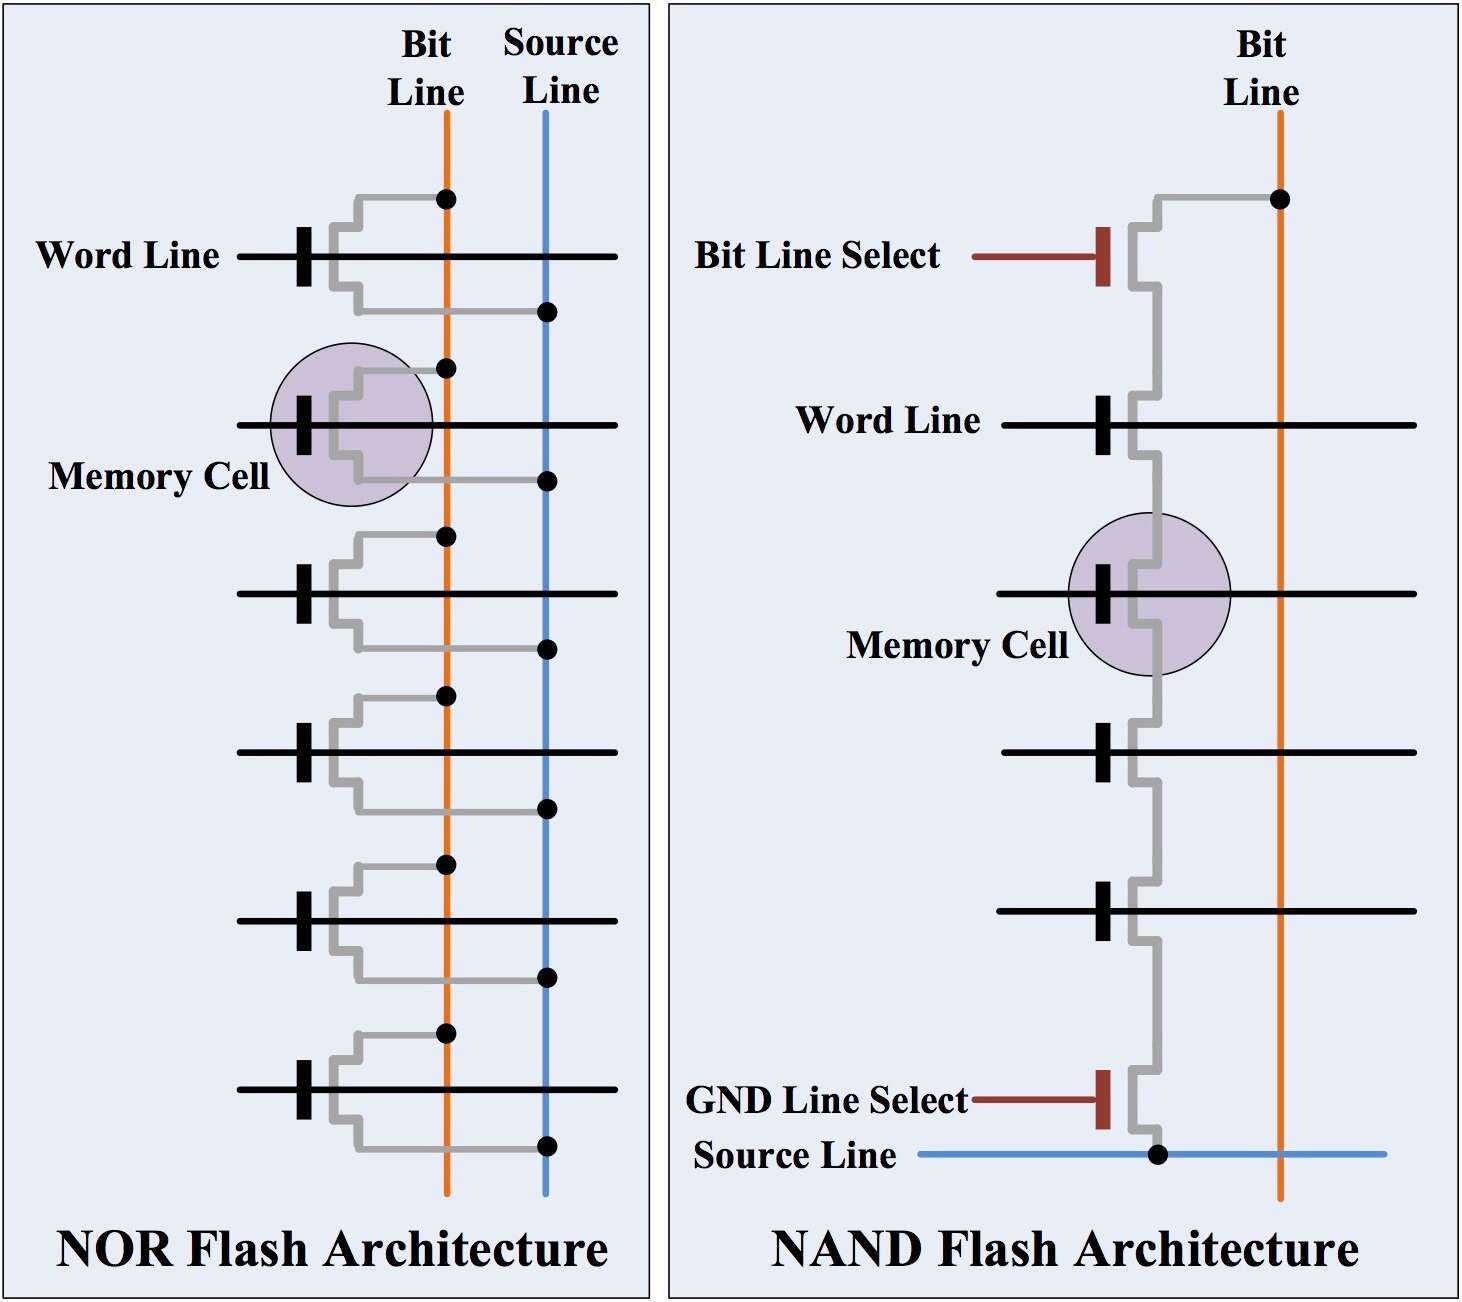
\includegraphics[width=0.8\linewidth]{res/nor-vs-nand-flash.jpg}
    \caption{NOR 플래시와 NAND 플래시의 원리.}
    \label{fig:nor-vs-nand-flash}
\end{figure}

NOR 플래시의 경우 각 MOSFET이 NOR 게이트의 트랜지스터 단 다이어그램과 같이 source 라인과 bit 라인 모두에 연결되어 있는 것을 볼 수 있다. 이 덕분에 NOR 플래시는 임의의 주소를 빠르게 읽어들일 수 있고, 메모리 셀의 수명과 상태를 100\% 정확하게 알 수 있다는 점이 특징이다. 하지만 그만큼 부피가 커지고, 가격이 비싸다는 단점이 있다.

반대로 NAND 플래시의 경우 각 MOSFET이 하나의 source 라인을 공유한다는 점을 알 수 있다. 필요한 연결의 개수가 적은 만큼 NAND 플래시는 부피가 작고, 가격이 싸다. 그러나 하나의 source를 여러 메모리 셀이 공유하는 NAND 플래시의 디자인상 완벽한 데이터 안정성을 보장할 수 없으며 읽기 속도가 조금 뒤떨어진다는 단점이 있다.

\question*{RAM의 구조 및 구동과정을 조사한 뒤 정리하시오.}

RAM은 \textit{Random Access Memory}의 약자로, 컴퓨터의 주기억장치로 사용되는 부품이다. 보통 프로그램이 실행 중에 선언되는 변수 또는 동적 할당되는 메모리가 모두 RAM에 저장되게 된다. RAM의 특징은 휘발성 메모리라는 점으로, 전원이 끊기면 저장되어 있는 정보가 모두 사라진다는 점이다.

우리가 컴퓨터에서 자주 볼 수 있는 RAM의 종류는 DRAM{\footnotesize Dynamic RAM}인데, 이 DRAM은 보통 MOS 축전기를 사용하여 제작된다. 각 축전기를 충전하거나 방전시키는 것으로 1 또는 0 값을 저장한다는 점이 특징이다.

\begin{figure}[ht]
    \centering
    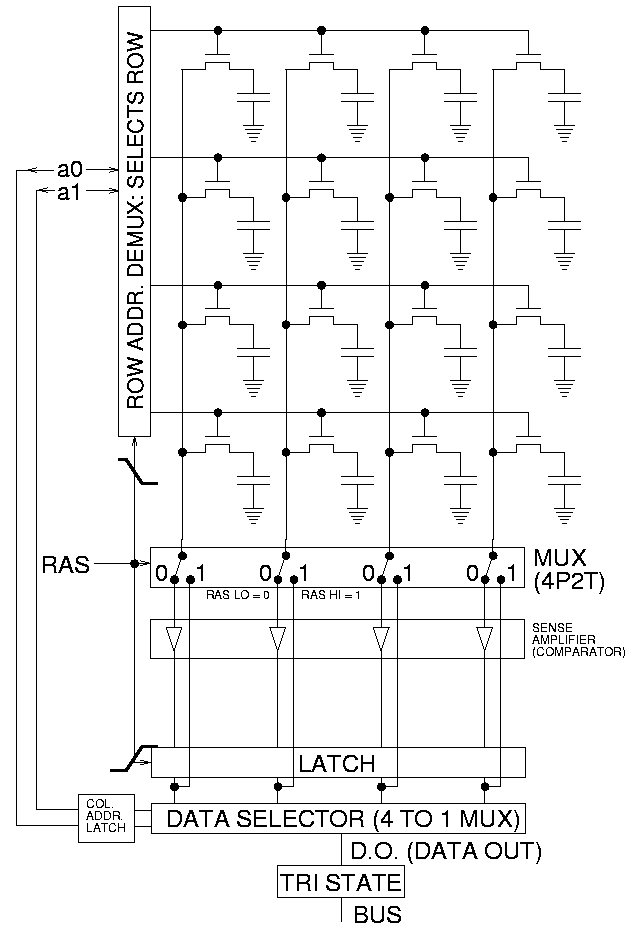
\includegraphics[width=0.8\linewidth]{res/square-dram-array.png}
    \caption{기본적인 2D DRAM 배열의 구조.}
    \label{fig:2d-dram-diagram}
\end{figure}

\end{document}